\chapter{\label{chap:results}Resultados}

\section{Cenário \textit{Low-rise}}

\lipsum[1]

\begin{table}[htb!]
\centering
\caption{Parâmetros do cenário \textit{Low-rise}.}
\label{tab:results:lowrise:params}
\begin{tabular}{|r|l|}
\hline
\textbf{Propriedade}          & \textbf{Valor}       \\ \hline
\textit{Nome}                 & Low-rise             \\ \hline
\textit{Duração (s)}          & 43200                \\ \hline
\textit{Semente}              & 54TH7hboAG1iOsDIDhJp \\ \hline
\textit{Elevatores}           & 2                    \\ \hline
\textit{Capacidade}           & 6                    \\ \hline
\textit{Andares}              & 11                   \\ \hline
\textit{Horizonte (planning)} & 5                    \\ \hline
\end{tabular}
\end{table}

\begin{table}[htb!]
\centering
\caption{Resultados obtidos da simulação do cenário \textit{Low-rise}.}
\label{tab:results:lowrise}
\begin{tabular}{|l|r|r|r|r|r|r|}
\hline
\multicolumn{1}{|c|}{\textbf{}}                 & \multicolumn{3}{c|}{\textbf{Tempo de Espera}}                                                                    & \multicolumn{3}{c|}{\textbf{Tempo de Jornada}}                                                                                                                       \\ \hline
\textbf{Estratégia} & \multicolumn{1}{c|}{\textit{Médio}} & \multicolumn{1}{c|}{\textit{Desvio}} & \multicolumn{1}{c|}{\textit{Total}} & \multicolumn{1}{c|}{\textit{Médio}}                   & \multicolumn{1}{c|}{\textit{Desvio}}                  & \multicolumn{1}{c|}{\textit{Total}}                  \\ \hline
\textit{Simple / Random}          & \cellcolor[HTML]{FD6864}5.4064      & \cellcolor[HTML]{FD6864}4.1792       & \cellcolor[HTML]{FD6864}16933       & \cellcolor[HTML]{FD6864}{\color[HTML]{000000} 4.4949} & 2.8676                                                & \cellcolor[HTML]{FD6864}{\color[HTML]{000000} 14078} \\ \hline
\textit{Planning / Random}        & \cellcolor[HTML]{67FD9A}3.1580      & \cellcolor[HTML]{67FD9A}2.8688       & \cellcolor[HTML]{67FD9A}9891        & 4.4713                                                & \cellcolor[HTML]{FD6864}{\color[HTML]{000000} 3.0005} & 14004                                                \\ \hline
\textit{Simple / NN}              & 3.5144                              & \cellcolor[HTML]{FFFFFF}3.5768       & 11007                               & 4.4700                                                & 2.8565                                                & 14000                                                \\ \hline
\textit{Planning / NN}            & 3.2273                              & 3.0515                               & 10108                               & 4.4770                                                & 2.9796                                                & 14022                                                \\ \hline
\textit{Simple / BNN}             & 3.3547                              & 3.2931                               & 10507                               & 4.4674                                                & 2.9163                                                & 13992                                                \\ \hline
\textit{Planning / BNN}           & 3.1830                              & 2.9150                               & 9969                                & \cellcolor[HTML]{67FD9A}4.4623                        & \cellcolor[HTML]{FFFFFF}2.9787                        & \cellcolor[HTML]{67FD9A}13976                        \\ \hline
\textit{Simple / Weighted}        & 3.7149                              & 3.8036                               & 11635                               & 4.4719                                                & \cellcolor[HTML]{67FD9A}2.7997                        & 14006                                                \\ \hline
\textit{Planning / Weighted}      & 3.2529                              & 3.0760                               & 10188                               & 4.4789                                                & 2.9714                                                & 14028                                                \\ \hline
\end{tabular}
\end{table}

\begin{figure}[htb]
  \centering
  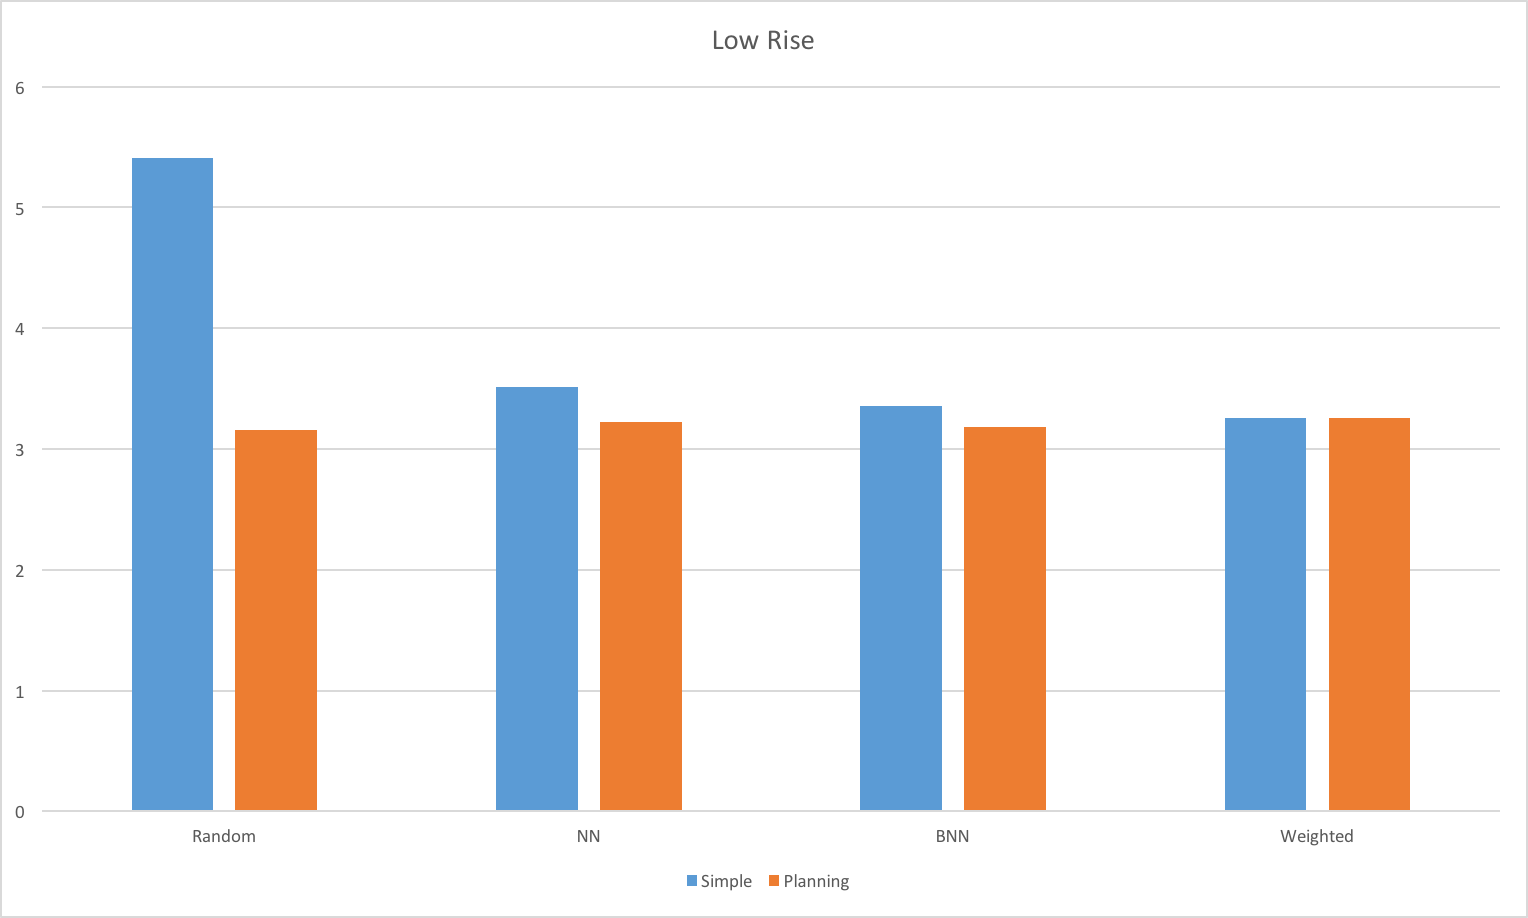
\includegraphics[scale=0.5]{img/chart-averages-low-rise}
  \caption{Comparação do tempo médio de espera com as diferentes estratégias
    para o cenário \textit{Low Rise}}
  \label{fig:result:average:low-rise}
\end{figure}

\section{Cenário \textit{High-rise}}

\lipsum[1]

\begin{table}[htb!]
\centering
\caption{Parâmetros do cenário \textit{High-rise}.}
\label{tab:results:highrise:params}
\begin{tabular}{|r|l|}
\hline
\textbf{Propriedade}          & \textbf{Valor}       \\ \hline
\textit{Nome}                 & High-rise            \\ \hline
\textit{Duração (s)}          & 43200                \\ \hline
\textit{Semente}              & w9JwgykwejtoL2icSgHo \\ \hline
\textit{Elevatores}           & 8                    \\ \hline
\textit{Capacidade}           & 10                   \\ \hline
\textit{Andares}              & 39                   \\ \hline
\textit{Horizonte (planning)} & 2                    \\ \hline
\end{tabular}
\end{table}

\begin{table}[htb!]
\centering
\caption{Resultados obtidos da simulação do cenário \textit{High-rise}.}
\label{tab:results:highrise}
\begin{tabular}{|l|r|r|r|r|r|r|}
\hline
\multicolumn{1}{|c|}{\textbf{}}                 & \multicolumn{3}{c|}{\textbf{Tempo de Espera}}                                                                    & \multicolumn{3}{c|}{\textbf{Tempo de Jornada}}                                                                                                                       \\ \hline
\textbf{Estratégia} & \multicolumn{1}{c|}{\textit{Médio}} & \multicolumn{1}{c|}{\textit{Desvio}} & \multicolumn{1}{c|}{\textit{Total}} & \multicolumn{1}{c|}{\textit{Médio}}                   & \multicolumn{1}{c|}{\textit{Desvio}}                  & \multicolumn{1}{c|}{\textit{Total}}                  \\ \hline
\textit{Simple / Random}          & 25.9981                         & 28.0464                         & 190124                          & \cellcolor[HTML]{FD6864}15.2595 & 14.9190                         & \cellcolor[HTML]{FD6864}111593  \\ \hline
\textit{Planning / Random}        &  8.8829                         & 16.5500                         &  64961                          & 15.1742                         & 12.0139                         & 110969                          \\ \hline
\textit{Simple / NN}              & 20.3395                         & 37.1902                         & 148743                          & 15.0993                         & 11.4479                         & 110421                          \\ \hline
\textit{Planning / NN}            &  9.9824                         & 19.4451                         &  73001                          & 15.1991                         & 11.4878                         & 111151                          \\ \hline
\textit{Simple / BNN}             & 13.5243                         & 23.5950                         &  98903                          & 15.0550                         & \cellcolor[HTML]{67FD9A}10.2476 & 110097                          \\ \hline
\textit{Planning / BNN}           & \cellcolor[HTML]{67FD9A}8.8202  & \cellcolor[HTML]{67FD9A}16.1712 & \cellcolor[HTML]{67FD9A} 64502  & 15.0982                         & 11.9491                         & 110413                          \\ \hline
\textit{Simple / Weighted}        & \cellcolor[HTML]{FD6864}31.0373 & \cellcolor[HTML]{FD6864}54.5909 & \cellcolor[HTML]{FD6864}226976  & \cellcolor[HTML]{67FD9A}14.9915 & \cellcolor[HTML]{FD6864}18.9700 & \cellcolor[HTML]{67FD9A}109633  \\ \hline
\textit{Planning / Weighted}      & 11.3271                         & 22.3406                         &  82835                          & 15.1173                         & 10.8752                         & 110553                          \\ \hline
\end{tabular}
\end{table}

\begin{figure}[htb]
  \centering
  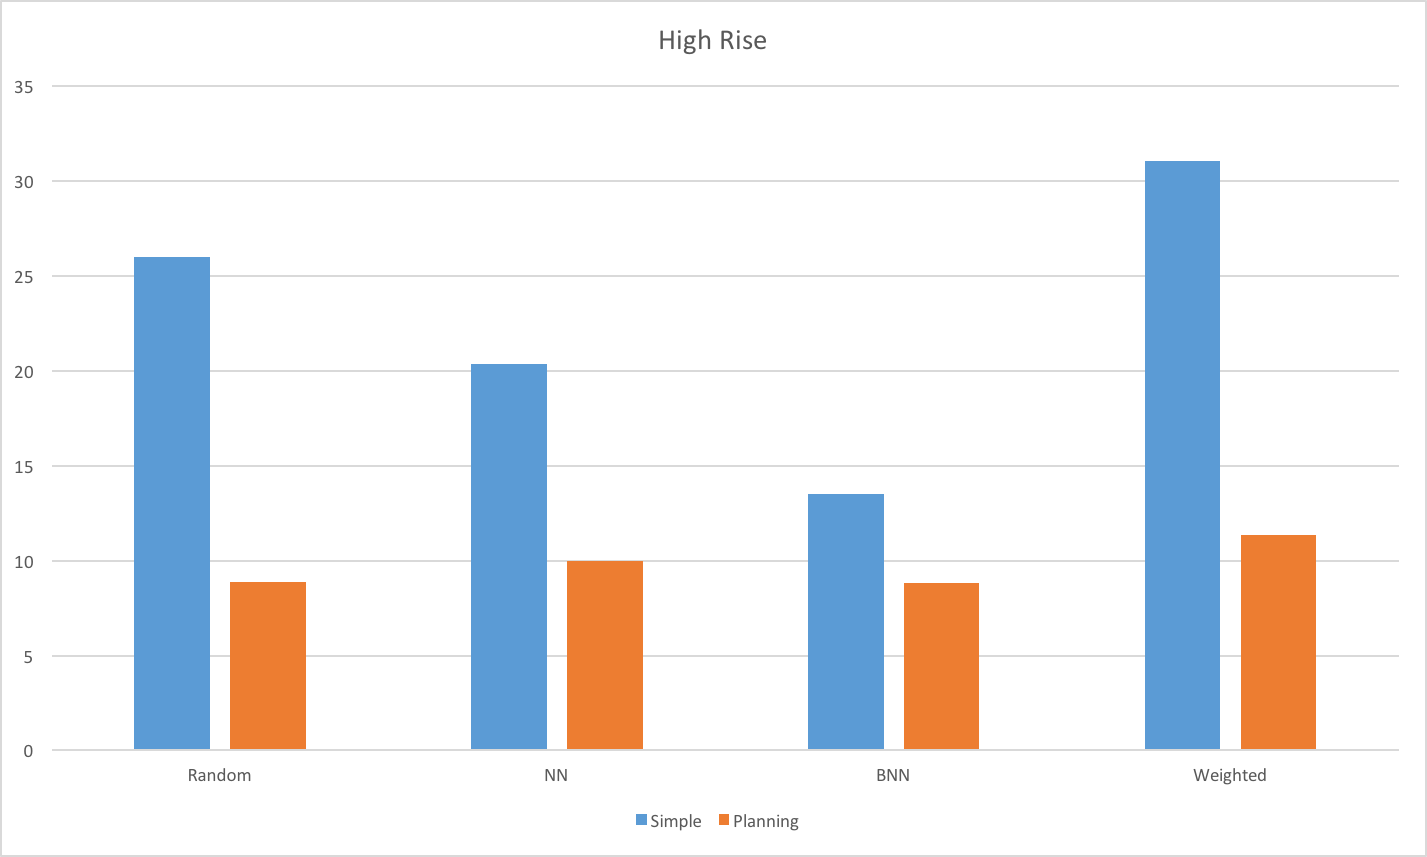
\includegraphics[scale=0.5]{img/chart-averages-high-rise}
  \caption{Comparação do tempo médio de espera com as diferentes estratégias
    para o cenário \textit{High Rise}}
  \label{fig:result:average:high-rise}
\end{figure}

\section{Cenário \textit{Skyscraper}}

\lipsum[1]

\begin{table}[htb!]
\centering
\caption{Parâmetros do cenário \textit{Skyscraper}.}
\label{tab:results:skyscraper:params}
\begin{tabular}{|r|l|}
\hline
\textbf{Propriedade}          & \textbf{Valor}       \\ \hline
\textit{Nome}                 & Skyscraper           \\ \hline
\textit{Duração (s)}          & 43200                \\ \hline
\textit{Semente}              & NimatYvEnU9QeE3GkF4J \\ \hline
\textit{Elevatores}           & 16                   \\ \hline
\textit{Capacidade}           & 12                   \\ \hline
\textit{Andares}              & 163                  \\ \hline
\textit{Horizonte (planning)} & 2                    \\ \hline
\end{tabular}
\end{table}

\begin{table}[htb!]
\centering
\caption{Resultados obtidos da simulação do cenário \textit{Skyscraper}.}
\label{tab:results:skyscraper}
\begin{tabular}{|l|r|r|r|r|r|r|}
\hline
\multicolumn{1}{|c|}{\textbf{}}                 & \multicolumn{3}{c|}{\textbf{Tempo de Espera}}                                                                    & \multicolumn{3}{c|}{\textbf{Tempo de Jornada}}                                                                                                                       \\ \hline
\textbf{Estratégia} & \multicolumn{1}{c|}{\textit{Médio}} & \multicolumn{1}{c|}{\textit{Desvio}} & \multicolumn{1}{c|}{\textit{Total}} & \multicolumn{1}{c|}{\textit{Médio}}                   & \multicolumn{1}{c|}{\textit{Desvio}}                  & \multicolumn{1}{c|}{\textit{Total}}                  \\ \hline
\textit{Simple / Random}          & \cellcolor[HTML]{FD6864}442.2165  & \cellcolor[HTML]{FD6864}1775.3156   & \cellcolor[HTML]{FD6864}10538904  & 54.7816                         & \cellcolor[HTML]{FD6864}389.3520  & 1305554                         \\ \hline
\textit{Planning / Random}        & \cellcolor[HTML]{67FD9A}74.9480   & \cellcolor[HTML]{67FD9A}198.3020    & \cellcolor[HTML]{67FD9A}1786161   & \cellcolor[HTML]{FD6864}59.1500 & \cellcolor[HTML]{67FD9A}46.7326   & \cellcolor[HTML]{FD6864}1409662 \\ \hline
\textit{Simple / NN}              & 343.5988                          & 1426.3821                           &  8188647                          & 54.9789                         & 291.2258                          & 1310258                         \\ \hline
\textit{Planning / NN}            & 103.6866                          &  307.8567                           &  2471058                          & 57.5756                         &  62.5268                          & 1372142                         \\ \hline
\textit{Simple / BNN}             & 287.1803                          & 1137.2342                           &  6844080                          & 55.0124                         & 235.4007                          & 1311056                         \\ \hline
\textit{Planning / BNN}           &  87.0986                          &  239.3584                           &  2075733                          & 58.2380                         &  51.9262                          & 1387928                         \\ \hline
\textit{Simple / Weighted}        & 293.8791                          & 1018.5118                           &  7003726                          & \cellcolor[HTML]{67FD9A}54.6163 & 242.3278                          & \cellcolor[HTML]{67FD9A}1301616 \\ \hline
\textit{Planning / Weighted}      &  99.2689                          &  314.6784                           &  2365776                          & 57.4469                         &  59.3754                          & 1369074                         \\ \hline
\end{tabular}
\end{table}

\begin{figure}[htb]
  \centering
  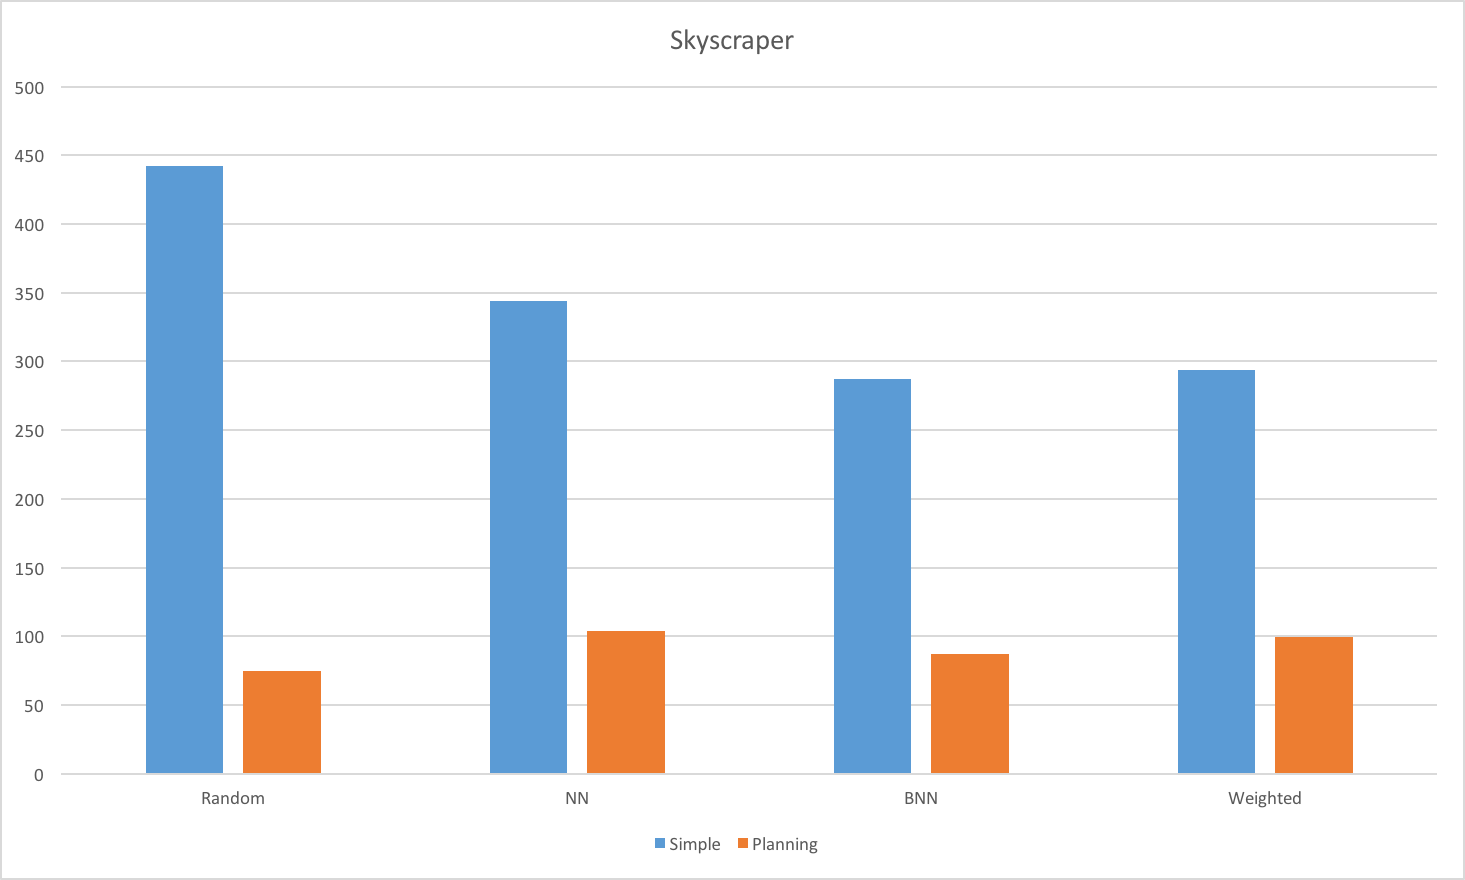
\includegraphics[scale=0.5]{img/chart-averages-skyscraper}
  \caption{Comparação do tempo médio de espera com as diferentes estratégias
    para o cenário \textit{Skyscraper}}
  \label{fig:result:average:skyscraper}
\end{figure}